\documentclass[a4paper,11pt,twocolumn]{article}
\usepackage[utf8]{inputenc}
\usepackage[T1]{fontenc}
\usepackage[spanish]{babel}
\usepackage[margin=1.75cm]{geometry}
\usepackage{lmodern}
\usepackage{graphicx}
\usepackage{booktabs}
\usepackage[numbers]{natbib}
\usepackage[colorlinks=true,linkcolor=blue,citecolor=blue]{hyperref}
\usepackage[labelfont=bf]{caption}
\usepackage{float}
\usepackage{sectsty}
\sectionfont{\sffamily\large}

\newcommand{\unit}[1]{\ensuremath{\,\mathrm{#1}}}

\title{\sffamily\bfseries @title}
\author{\sffamily @author}
\date{\sffamily\today}

\begin{document}
\maketitle

\section*{Introducción}

Este reporte preliminar de tsunami de origen lejano ha sido elaborado en forma automática por el modelo numérico TSDHN-2022. Las dimensiones de la fuente sísmica se calculan a partir de las ecuaciones de Papazachos et al. (2004). El mecanismo focal del terremoto se toma de la base de datos del Global CMT. El campo de deformación se obtiene a partir de las ecuaciones analíticas de Okada (1992).

La simulación de la propagación del tsunami se realiza con el modelo numérico TUNAMI, modelo lineal y en coordenadas esféricas (Imamura et al., 2006). La grilla batimétrica computacional abarca el Océano Pacífico, con una resolución de 4 min o 240 s. El cálculo de las isócronas de tiempos de arribo para el Océano Pacífico se realizó con el modelo Tsunami Travel Time (Wessel, 2009).

Se han colocado 3 mareógrafos virtuales en los puertos de Talara, Callao y Matarani. Se utilizó la ley de Green para la corrección de la amplitud de los mareogramas, debido a que los nodos computacionales no coinciden necesariamente con la ubicación de las estaciones mareográficas costeras (Satake, 2015).

\textbf{Nota:} El resultado del modelo TSDHN-2022 es una estimación referencial y debe ser utilizado para obtener los parámetros de tsunamis de origen lejano, es decir fuera de las fronteras del litoral de Perú. Para eventos de origen cercano, se debe utilizar el modelo Pre-Tsunami (Jimenez et al., 2018).

\section*{Análisis}

El cuadro 1 muestra los parámetros hipocentrales del terremoto.

\begin{table}[H]
  \centering
  \begin{tabular}{@@{}l c@@{}}
    \toprule
    \textbf{Parámetro} & \textbf{Valor} \\
    \midrule
    Latitud     & @lat\unit{^\circ} \\
    Longitud    & @lon\unit{^\circ} \\
    Profundidad & @depth\unit{km} \\
    Magnitud    & @magnitude\unit{M_w} \\
    \bottomrule
  \end{tabular}  
\end{table}

El cuadro 2 muestra los parámetros del mecanismo focal del terremoto.

\begin{table}[H]
  \centering
  \begin{tabular}{@@{}lc@@{}}
    \toprule
    \textbf{Parámetro} & \textbf{Valor} \\
    \midrule
    Strike & @strike\unit{^\circ} \\
    Dip    & @dip\unit{^\circ} \\
    Rake   & @rake\unit{^\circ} \\
    \bottomrule
  \end{tabular}
\end{table}

La figura \ref{fig:maxola} muestra el mapa de propagación de la máxima energía, la ubicación del epicentro está representado por la esfera focal y las estaciones mareográficas están representadas por los triángulos azules.

\begin{figure}[H]
  \centering
  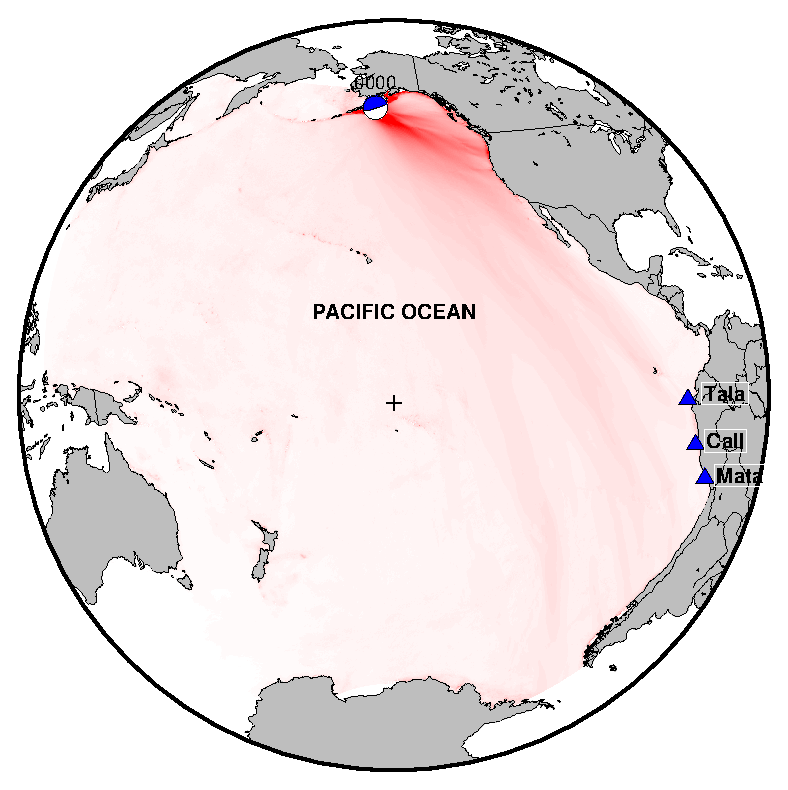
\includegraphics[width=.95\linewidth]{maxola.eps}
  \caption{Mapa de máxima altura de propagación del tsunami. La esfera focal representa el epicentro. Los triángulos azules representan a las estaciones mareográficas.}
  \label{fig:maxola}
\end{figure}

La figura \ref{fig:ttt} muestra las isócronas de los tiempos de arribo del tsunami para todo el Océano Pacífico. 

\begin{figure}[H]
  \centering
  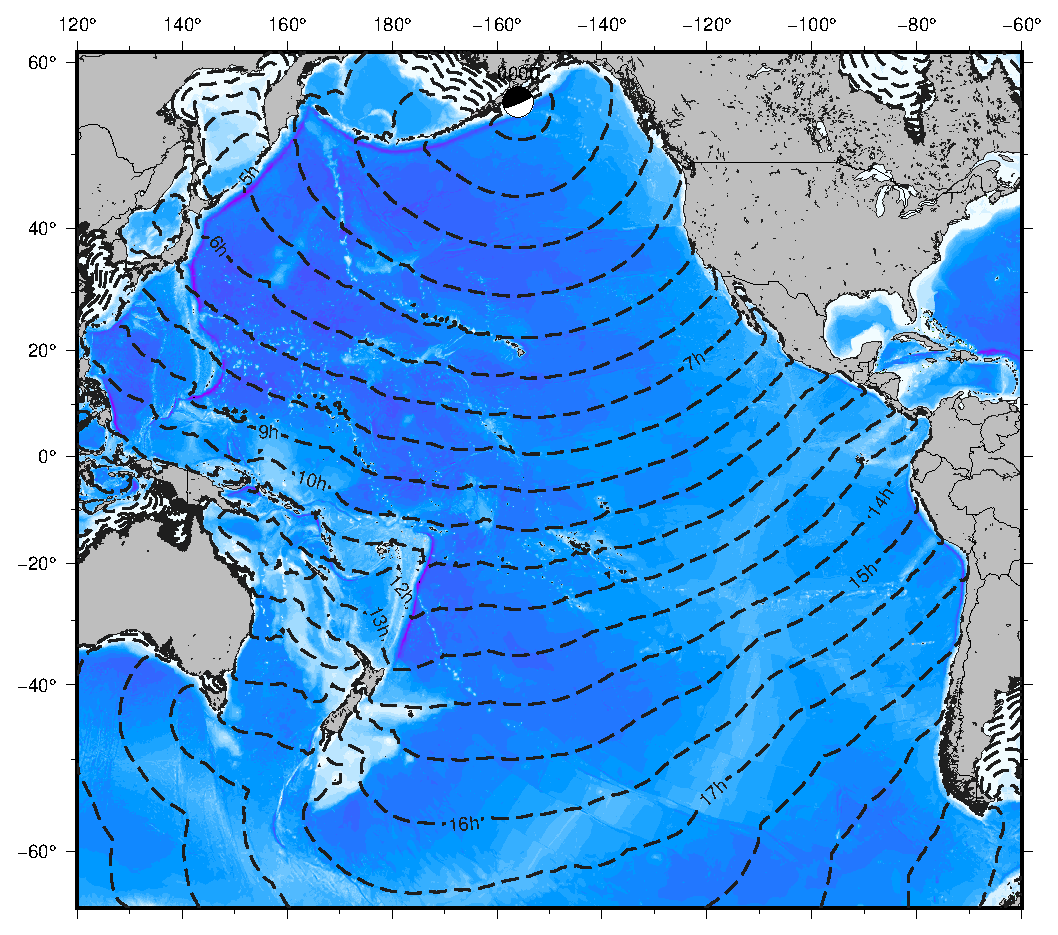
\includegraphics[width=\linewidth]{ttt.eps}
  \caption{Mapa de tiempo de arribo del tsunami. La esfera focal representa el epicentro.}
  \label{fig:ttt}
\end{figure}

La figura \ref{fig:mareogramas} muestra los mareogramas simulados para las estaciones del litoral del Perú, de norte a sur: Talara, Callao y Matarani.

\begin{figure}[H]
  \centering
  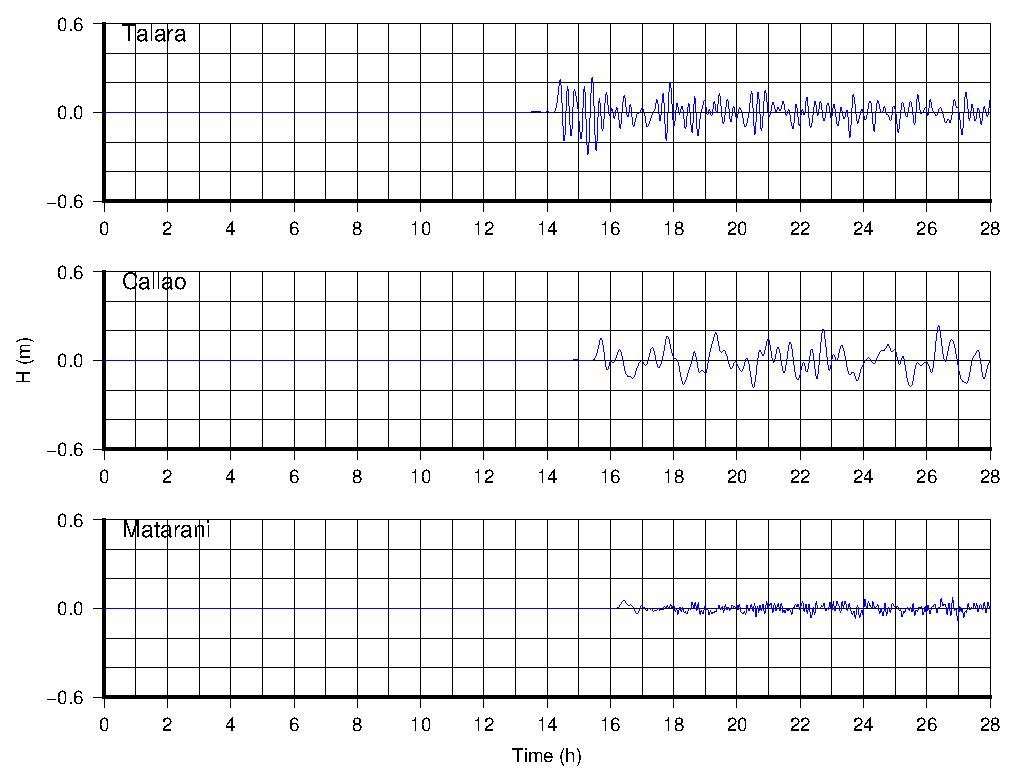
\includegraphics[width=\linewidth]{mareograma.eps}
  \caption{Mareogramas simulados en las estaciones de Talara, Callao y Matarani.}
  \label{fig:mareogramas}
\end{figure}

El cuadro 3 muestra los valores de los tiempos de arribo y la máxima altura del tsunami en las estaciones mareográficas del litoral peruano.

\begin{table}[H]
  \centering
  \begin{tabular}{@@{}lcc@@{}}
    \toprule
    \textbf{Estación} & \textbf{Tiempo de arribo} & \textbf{Máximo (m)} \\
    \midrule
    @station1_name & @station1_time & @station1_max \\
    @station2_name & @station2_time & @station2_max \\
    @station3_name & @station3_time & @station3_max \\
    \bottomrule
  \end{tabular}
  \caption{Tiempo de arribo (hh:mm) y máxima amplitud del tsunami}
\end{table}

\newpage 
\begin{thebibliography}{99}
\bibitem{1} B. Papazachos, E. Scordilis, C. Panagiotopoulus and G. Karakaisis. Global relations between seismic fault parameters and moment magnitude of earthquakes. Bulletin of Geological Society of Greece, vol XXXVI, pp 1482-1489 (2004).
\bibitem{2} Y. Okada. Internal deformation in a half space. Bull. Seismol. Soc. Am. 82(2) 1018-1040 (1992).
\bibitem{3} F. Imamura, A. Yalciner and G. Ozyurt. Tsunami Modelling Manual (TUNAMI model). Tohoku University, Sendai. (2006).
\bibitem{4} P. Wessel. Analysis of observed and predicted tsunami travel times for the Pacific and Indian Oceans. Pure Appl. Geophys., vol 166, pp 301--324 (2009).
\bibitem{5} K. Satake. Tsunamis, inverse problem of. Encyclopedia of Complexity and Systems Science, pp 1--20 (2015).
\bibitem{6} C. Jimenez, C. Carbonel and J. Rojas. Numerical procedure to forecast the tsunami parameters from a database of pre-simulated seismic unit sources. Pure Appl. Geophys., vol 175, pp 1473--1483 (2018).
\end{thebibliography}

\end{document}
